\documentclass[11pt]{article}
\usepackage{graphicx} % Required for inserting images
\usepackage[top=2.5cm, bottom=2cm, left=2cm, right=2cm]{geometry}
\usepackage[T1]{fontenc}
\usepackage{hyperref}
\usepackage[utf8]{inputenc}
\usepackage{multirow}
\usepackage{subcaption}
\usepackage{booktabs}
\usepackage{bookmark}
\usepackage{graphicx}
\usepackage{setspace}
\setlength{\parindent}{0in}
\usepackage{physics}
\usepackage{tikz}
\usepackage{tikz-3dplot}
\usepackage[outline]{contour} % glow around text
\usepackage{xcolor}
\usepackage{float}
\usepackage{makeidx}
\usepackage{fancyhdr}
\usepackage{pgfplots}
\usepackage{amsmath}
\pgfplotsset{compat=1.18}
\usepackage{caption}
\usepackage[english,catalan]{babel}
\setlength{\parskip}{11pt}
\usepackage{xcolor}
\usepackage{listings}
\usepackage{marginnote}
\usepackage{siunitx}
\usepackage{framed}
\usepackage{ulem}


\begin{document}

\tableofcontents
\newpage
\vspace{10em}

{\huge \textbf{Pràctica 6}}  % Títol petit en negreta

\vspace{0.5em}  % Espai vertical

{\Huge \textbf{Feixos de raigs catòdics}}  % Títol gran

\begin{abstract}
     En aquesta pràctica s'estudia el comportament d'un feix de raigs catòdics sota un camp elèctirc i un camp magnètic amb l'objectiu de determinar les propietats de les partícules que els conformen. Concretament, analitzant les desviacions del feix dels raigs sota aquests camps s'obté la relació entre la càrrega i la massa de les partícules que ens permet determinar que són electrons.
\end{abstract}

\section{Introducció Teòrica}
En aquesta pràctica estudiarem com es desvia el feix de raigs catòdics sota el camp elèctric generat per un condensador i el camp magnètic generat per unes bobines de Helmoholtz. A través de les equacions d'aquests, podrem determinar propietats de les partícules que conformen els raigs. Concretament, els objectius que ens plantegem són:

\begin{list}{$\ast$}{\leftmargin=1em}
    \item Caracteritzar el camp elèctric generat pel condensador no ideal que usem a l'experiment a través d'un factor experimental.
    \item Determinar i explicar el comportament dels raigs catòdics sota el camp elèctric i el camp magnètic. Estudiar-ho per diferents intencitats i potencials aplicats als generadors de camp.
    \item Determinar, amb dos mètodes diferents, de què estan fets els raigs catòdics trobant la relació entre la càrrega i la massa de les seves partícules.
\end{list}


%DESV E
Primerament, estudiarem la desviació del feix degut a un camp elèctric perpendicular a la velocitat; aplicant una diferència de potencial $V_p$ entre dues plaques plano-paral·leles. Degut a què la distància entre plaques $d$ (= 54 mm) és de l'ordre del tamany d'aquestes, no podem considerar el sistema com un condensador de plaques plano-paral·leles ideal amb un camp uniforme $E=V/d$. En comptes, seguirem considerant-lo uniforme però modificarem l'expressió mitjançant una constant $k$ que tindrà en compte els efectes de vorada i que trobarem experimentalment.
\begin{equation}
    E = \frac{kV_p}{d}
    \label{eq: Camp E}
\end{equation}

Si les partícules de les quals està format els raigs catòdics (de massa $m$) tenen càrrega elèctrica $q$, aquestes es desviaran cap a un dels dos elèctrodes; al càtode si són negatives i a l'ànode si són positives. I la trajectòria que seguiran serà una paràbola parametritzada per l'Eq. (\ref{eq: trajectoria}), ja que el camp és uniforme i en direcció $y$.
\begin{align}    \label{eq: trajectoria}
    &x = v_0 t      &y = -\frac{qEt^2}{2m}
\end{align}

On $v_0$ és la velocitat en direcció $x$ que tenen inicialment les partícules al sortir del filament.
Donat que un cop emeses les partícules, aquestes es veuen accelerades degut al voltatge aplicat $V_a$; per conservació de l'energia, la velocitat ha de ser:
\begin{equation}
    \frac{1}{2}mv_0^2=qV_a
    \label{eq: Energia}
\end{equation}

Tot i això, no es pot veure el moviment d'una partícula individual en funció del temps, sinó que es veu una corba formada per moltes partícules en diferents moments de la trajectòria. L'expressió d'aquesta corba com una funció de $x$ ($y$ = $f(x)$)  s'obtè combinant les Eqs. (\ref{eq: Camp E}), (\ref{eq: trajectoria}) i (\ref{eq: Energia}):
\begin{equation}
    y = \frac{kV_px^2}{4dV_a}
    \label{eq: parabola}
\end{equation}

Per últim, queda determinar experimentalment la constant $k$ a partir del pendent $m$ de la recta de regressió lineal de $y$ en funció de $x^2$ i de l'equació (\ref{eq: parabola}):
 \begin{equation}
      k =\frac{4mdV_a}{V_p}
      \label{eq: k}
 \end{equation}

%DESV M
\vspace{1cm}

Per calcular el radi de corvatura i posteriorment la relació $\frac{q}{m}$ de les partícules dels raigs catòdics necessitem caracteritzar la trajectòria de les partícules carregades sota un camp magnètic uniforme. En l'experiment, el camp d'inducció magnètica està generat per unes bobines de Hemholtz que aproximadament produeixen el camp uniforme 
\begin{equation}
    \vec{B}=\frac{32\pi nI}{5\sqrt{5}r}\cross10^{-7} \quad \hat{z}\quad Wb/m^2.
    \label{eq: B}
\end{equation}
Per altra banda, la llei de Lorentz dicta que una partícula carregada negativament sota un camp d'inducció magnètica, $\vec{B}$, pateix una força
\begin{equation}
    \vec{F}=q\vec{v}\cross\vec{B}.
    \label{eq: Lorentz} 
\end{equation} 
En el nostre cas, $\vec{v}$ és perpendicular a $\vec{B }$ i, per tant, les partícules dels raigs catòdics seguiran una trajectòria circular d'equació
%Aquesta força, al ser sempre perpendicular a la velocitat i tenint en compte que en el nostre sistema la velocitat de les partícules carregades, $\vec{v}$, és perpendicular a $\vec{B }$ induirà un moviment circular a les partícules de radi R. La trajectòria de les partícules carregades del nostre sistema complirà
\begin{equation}
    R=\frac{x^2+y^2}{2y}.
    \label{eq: radi}
\end{equation}
On $R$ és el radi del cercle i hem agafag el centre de coordenades a l'inici del tub de raigs catòdics i l'eix $X$ del sistema paral·lel a la direcció de sortida dels raigs.

Ara, per calcular la relació entre la intensitat de corrent de les bobines de Helmoholtz i el radi de corvatura de les partícules cal igualar la força centrípeta a la força de Lorentz, i obtenim 
\begin{equation}
    Bqv=\frac{mv^2}{R}
    \label{eq: fc=fl}
\end{equation}
que combinada amb l'Eq. (\ref{eq: B}) ens dona la relació entre el radi i la intensitat de corrent
\begin{equation}
    R=K\frac{1}{I} \quad on \quad K=\frac{mv5\sqrt{5}r}{32\pi n}\cross 10^7.
    \label{eq: IvsR}
\end{equation}
Tenint en compte l'Eq. (\ref{eq: fc=fl}) i la llei de la conservació de l'energia mecànica, $qV_a = \frac{1}{2}mv^2$, s'obté 
\begin{equation}
    \frac{q}{m}=\frac{2V_a }{B^2R^2}
    \label{eq: q/m}
\end{equation}
que ens permetrà calcular la relació $\frac{q}{m}$ de les partícules.


\vspace{1cm}

Una altre manera de calcular la relació càrrega/massa de les partícules dels raigs catòdics és igualant forces elèctriques i magnètiques. Fent-ho, arribem a la següent equació:

\begin{equation}\label{eq: Fm=Fe}
    qE = qvB
\end{equation}

Amb la que es troba que la velocitat vindrà donada pel quocient:

\begin{equation}
    v = \frac{E}{B}
\end{equation}

Podem obtenir el radi de la trajectòria circular deguda només a la desviació magnètica com hem explicat prèviament.

De les Eqs \eqref{eq: Fm=Fe}, \eqref{eq: fc=fl} es pot deduir l'equació que emprem en la secció \ref{sec: desv_em} per a calcular la relació càrrega/massa a partir de les nostres dades experimentals:

\begin{equation}
    \frac{q}{m}=\frac{E}{RB^2}=\frac{kV_p}{dK^2I^2R}
\end{equation}

\newpage
\section{Mètode Experimental}

El procediment experimental seguit ha constat de diversos passos que estan explicades detalladament al guió de la pràctica. 
Primerament, s'ha aplicat una diferència de potencial al tub de raigs catòdics i s'ha fet visible el feix lluminós dels raigs. Tot seguit s'ha estudiat la desviació d'aquest feix al aplicar diferents valors de camp elèctric (generat per un condensador planoparal·lel) o magnètic (generat per unes bobines de Hemholt) ambdós uniformes i perpendiculars. Per poder determinar punts de la trajectòria del feix de raigs catòdics, hem fotografiat el raig usant un dispositiu mòbil i cobrint-nos amb un material opac per tal de tenir més contrast. Posteriorment, aquestes fotografies han estat processades digitalment.

En el cas del camp magnètic, per poder estudiar la relació entre el radi de corvatura del feix i la intensitat de corrent de les bobines de Helmholtz, s'ha fotografiat el raig per les següents intensitats:  $0.1A, 0.2A, 0.3A, 0.4A, 0.5A, 0.6A, 0.7A, 0.8A$. Igualment, per determinar la relació entre el radi de corbatura i el potencial aplicat hem usat els següents potencials: $2kV, 3kV, 4kV$ i $5kV$.

En aquest punt, mitjançant un dispositiu mòbil s'han fotografiat els diferents casos. Aleshores, s'ha processat cada imatge, ja a ordinador, amb un programa d'edició que permet ajustar les mesures del feix mitjançant els propis píxels de les fotografies comparats amb les marques de la regla. Es a dir, comptant aquests píxels i convertint-los a centímetres. Aquest doncs, ha estat el procediment seguit: triar a consciència diversos punts del feix i donar-ne la posició (x,y) més exacta possible, sempre sent possibles errors degut al processat de la fotografia o al desplaçament de píxels. Més precisament, s'ha aplicat una grid (cuadrícula) sobre els espais compresos entre cada marca de la regla, coincidint amb cada variació de 1 cm, per cada eix. Així, per cada una de les imatges s'ha establert una conversió píxel/cm. S'inclou un exemple gràfic (\ref{fig: ex_grid}) a continuació:

\begin{figure}[H]
    \centering
    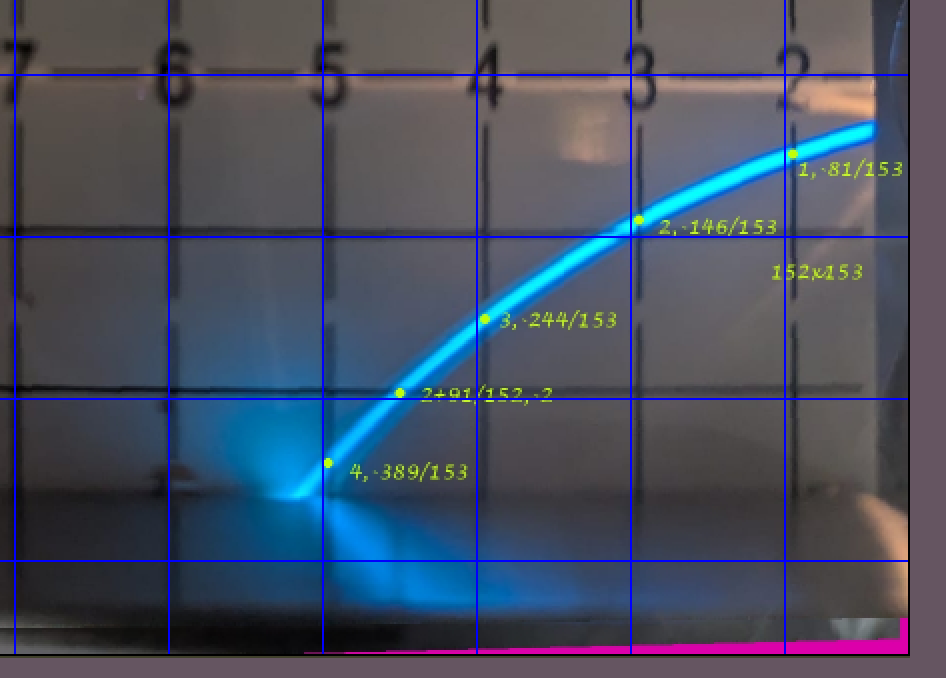
\includegraphics[scale=0.3]{Ex_grid.png}
    \caption{Imatge modificada després de l'aplicació de la grid corresponent amb la seva relació px/cm: 152/1 i 153/1.}
    \label{fig: ex_grid}
\end{figure}


Llavors, per cada un dels punts s'ha determinat la posició dins la grid comptant els píxels de separació amb la frontera del quadrat corresponent, i finalment, s'han convertit a centímetres. Amb aquests resultats, s'ha estudiat la desviació de la trajectòria; fet crucial pel desenvolupament de la prova, doncs les partícules del feix es poden identificar segons aquest comportament.

\newpage
\section{Resultats i discussió}

\section{Desviació electroestàtica}\label{sec: desv_electr}

En subministrar una diferència de potencial a les plaques s'observa com el raig es desvia cap al càtode\footnote{Les imatges de la desviació electroestàtica (Fig.(\ref{fig: Desv E})) es troben a l'annex (\ref{sec: imatges}) }. Per tant, les partícules de les què està compost els raigs catòdics tenen una càrrega negativa.

 Per comprovar que les trajectòries es tracten de paràboles hem fet una regressió de les $y$ en funció de les $x^2$, com es mostra a la figura (\ref{fig: Regressió Desv E}). Aquestes tenen els següents coeficients de correlació \footnote{Les regressions lineals en detall es troben a l'annex \ref{sec: Reg}}:
 r$^2$ = 0.9777, 0.9973, 0.9940, 0.9832. Confirmant que les partícules segueixen una trajectòria parabòlica.
\begin{figure}[h]
    \centering
    \begin{minipage}{0.75\textwidth}
    \centering
        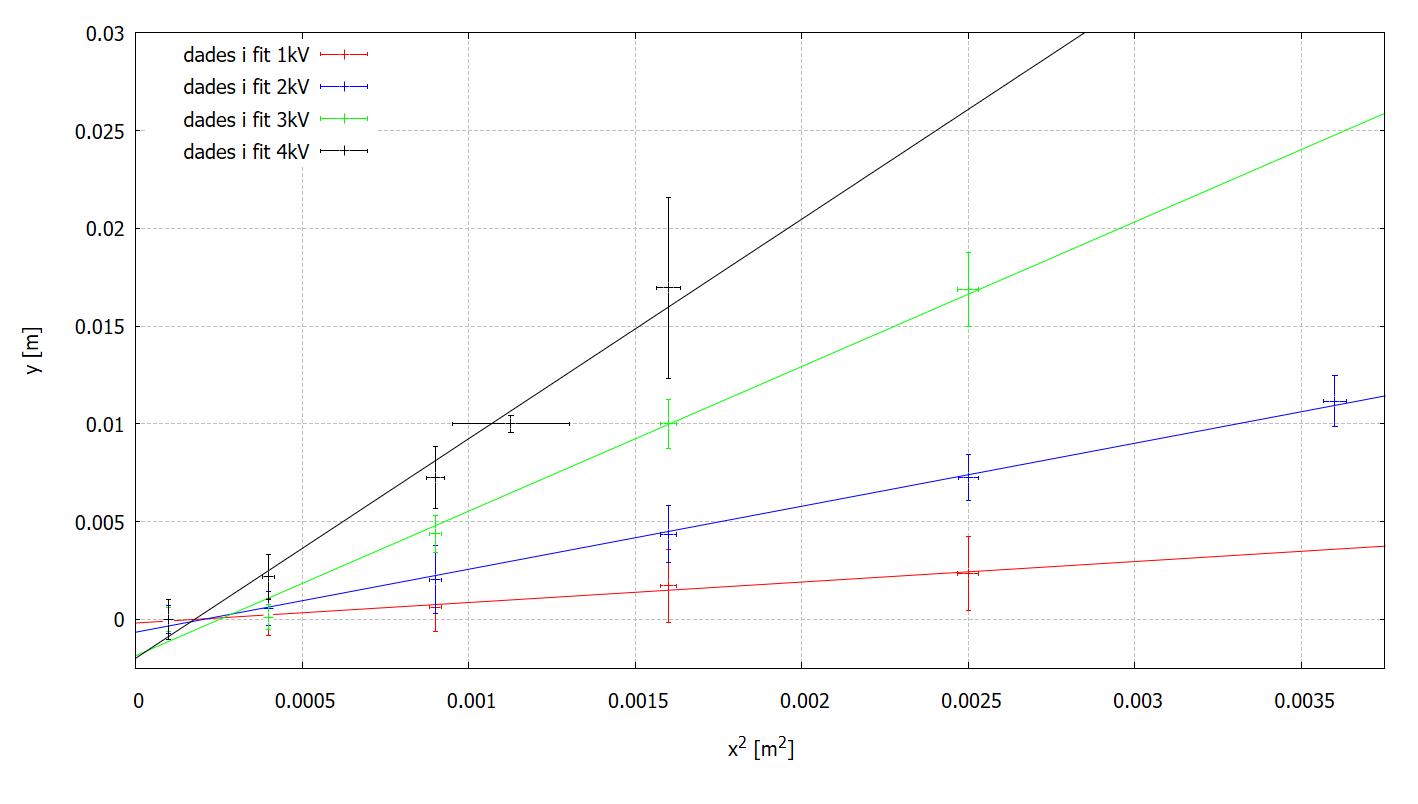
\includegraphics[width=1\linewidth]{Plot yvsx.PNG}
        \caption{Regressió de $y$ en funció de $x^2$  de la desviació deguda al camp elèctric}
        \label{fig: Regressió Desv E}
    \end{minipage}
\end{figure}

A la taula \ref{tab:kvsVp} podem observar els diferents valors que pren $k$ \footnote{El càlcul de les incerteses es mostra a l'anex \ref{sec: incerteses}} en funció del potencial entre plaques $V_p$, obtinguts a partir del pendent d'aquestes regressions lineals juntament amb l'Eq. (\ref{eq: k}). Observem que la $k$ no és constant i que augmenta amb la diferència de potencial. Fent una regressió lineal entre $V_p$ i $k$ obtenim que hi ha una relació lineal entre els dos amb un coeficient de correlació r$^2$ = 0.9737 i una equació de la recta: $k = 0.453 \cdot 10^{-3}\, V^{-1}  \cdot V_p + 0.45$.


\begin{figure}[h]
    \centering
    \begin{minipage}{0.45\textwidth} 
        \centering
        \begin{tabular}{|c|c|}
            \hline
            $V_p$ (V)	&	$k$	\\\hline
            (1000 ± 200)	&	(0.87 ± 0.64)   \\\hline
            (2000 ± 200)	&	(1.35 ± 0.22)	\\\hline
            (3000 ± 200)	&	(1.94 ± 0.25)	\\\hline
            (4000 ± 200)	&	(2.17 ± 0.26)	\\\hline           
        \end{tabular}
        \captionof{table}{Resultats experimentals de les constants $k$ del condensador per cada valor del potencial $V_p$.}
        \label{tab:kvsVp}
    \end{minipage}
\end{figure}


\subsection{Desviació magnetoestàtica}\label{sec: desv_magn}
Després de comprovar a la Secció \ref{sec: desv_electr} que les partícules dels ràigs catòdics tenen càrrega negativa, n'estudiarem la interecció amb el camp magnètic, substancialment uniforme, generat per unes bobines de Hemholtz. 
Al aplicar el camp, com era d'esperar, hem observat que els ràigs es corbaven i ens hem disposat a estudiar les dependències d'aquesta corba i el seu radi amb la intensitat del corrent de les bobines i amb el potencial dels raigs catòdics.

Per calcular el radi de la trajectòria de les partícules dels raigs catòdics en funció de la intensitat de corrent de les bobines hem usat l'Eq. (\ref{eq: radi}) que defineix el radi com el pendent de la recta de regressió entre $x^2+y^2$ i $2y$. A la Fig. (\ref{fig: regressio_1}) hem representat una selecció d'aquestes regressions i ja podem veure com a mesura que augmenta la intensitat, el pendent de la recta, és a dir el radi de les partícules, disminueix. 
\begin{figure}[H]
    \centering
    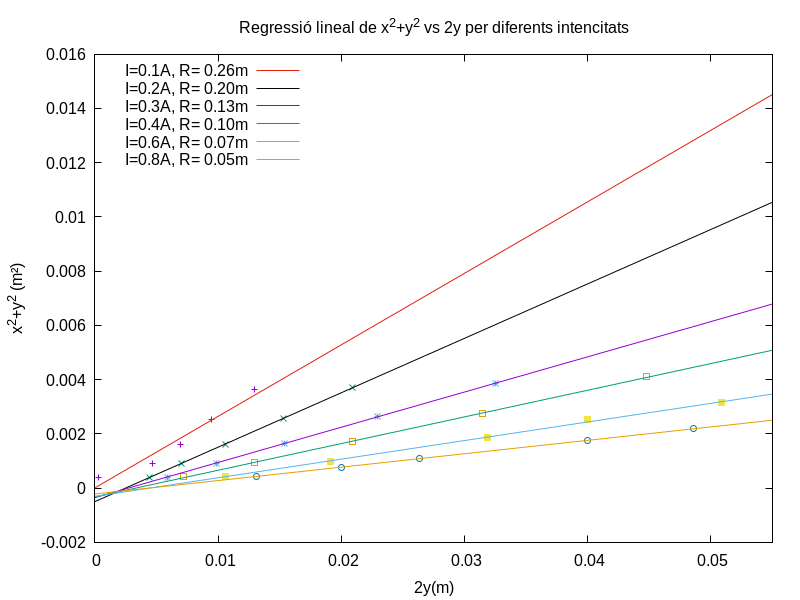
\includegraphics[scale=0.3]{regressio_1.png}
    \caption{Regressió per diverses intensitats de les bobines de Hemholtz de $x^2+y^2$ en front $2y$ on $y$ i $x$ són punts de la trajectòria dels raigs catòdics. La pendent de les rectes és el radi de corvatura de la trajectòria.}
    \label{fig: regressio_1}
\end{figure}
Aplicant diverses intensitats a les bobines de Helmholtz hem obtingut els radis de corvatura de la Taula \ref{tab:RvsI} que es pot trobar a l'annex conjuntament amb el càlcul d'incerteses. Amb aquestes dades (excloent l'última dada ja que té massa incertesa a causa de l'amplada del feix dels raigs) hem construit la gràfica de la Fig. (\ref{fig: RvsI}) on es mostra que la variació del radi corvatura és lineal amb la variació de la inversa de la intensitat. 
Al fer la regressió lineal del radi en funció de l'inversa de l'intensitat hem obtingut la recta
\begin{equation}
    y=x(0.03976\pm0.0006)+(0.0002\pm0.0016)
\end{equation}  
amb un coeficient de determinació de $r^2\approx0,99$. Per tant, la relació és certament lineal tot verificant la predicció de l'Eq.(\ref{eq: fc=fl}) ja que a més a més, l'ordenada a l'origen inclou el zero. El radi de corvatura és inversament proporcional a la intencitat a causa de què al augmentar la intensitat de les bobines de Hemholtz el camp d'inducció magnètica augmenta provocant que les partícules rebin més força centrípeta què alhora provoca que el radi de la trajectòria disminueixi.
\begin{figure}[h]
    \centering
    \begin{minipage}{0.45\textwidth}
        \centering
        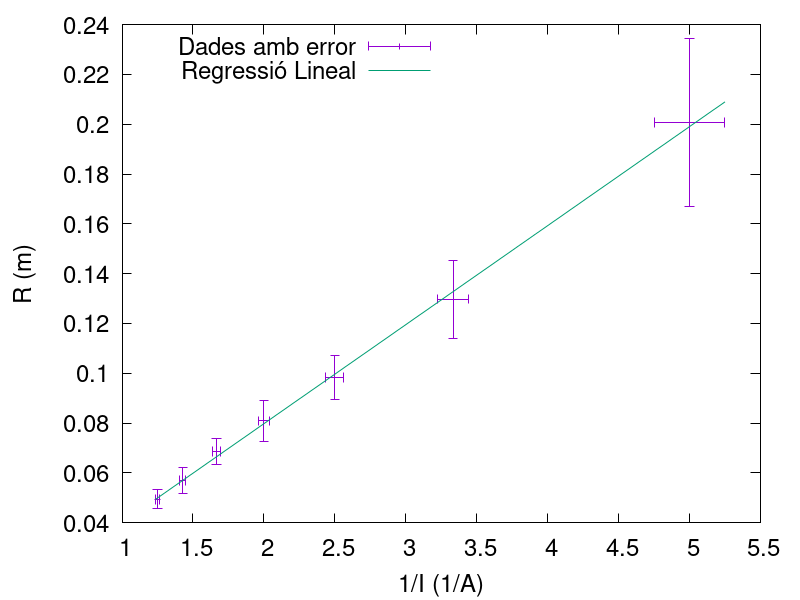
\includegraphics[width=\textwidth]{RvsI.png}
        \caption{Regressió de R en funció de $1/I$ excloent l'últim punt que perd la tendència.}
        \label{fig: RvsI}
    \end{minipage}
    \hfill
    \begin{minipage}{0.45\textwidth} 
        \centering
        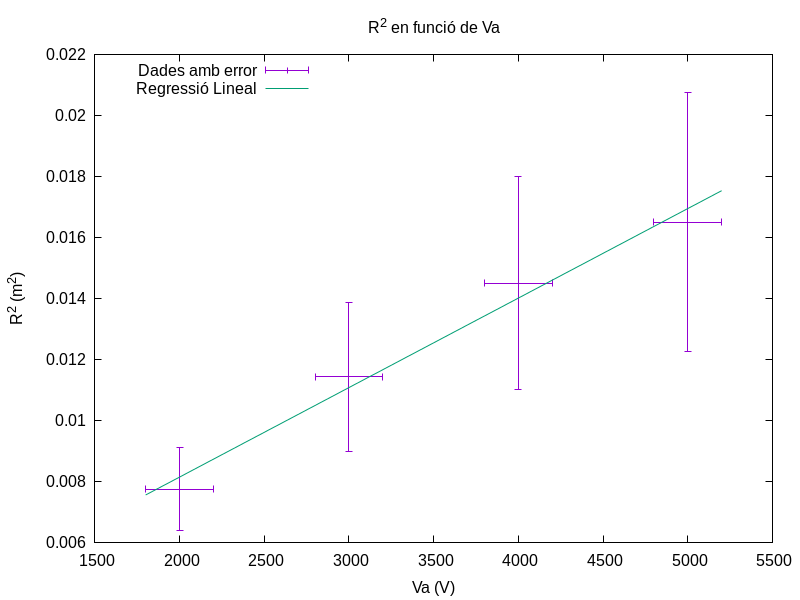
\includegraphics[width=\textwidth]{RvsVa.png}
        \caption{Regressió dels punts experimentals de $R^2$ en funció de $V_a$. Veiem que la relació és clarament lineal.}
        \label{fig: RvsVa}
    \end{minipage}
\end{figure}
Per calcular el radi de la trajectòria de les partícules dels raigs catòdics en funció del potencial d'acceleració d'aquestes usem l'Eq. (\ref{eq: radi}) que defineix el radi com el pendent de la recta de regressió entre $x^2+y^2$ i $2y$. Alicant diferents potencials a les bobines de Helmoholtz s'obtenen els radis de corvatura de la Taula \ref{tab:RvsVa} que es troba a l'annex. Amb aquestes dades hem construit la gràfica de la Fig. (\ref{fig: RvsVa}) on es mostra que la variació de $R$ és quadràtica amb la variació de $V_a$. Al fer la regressio lineal de $R^2$ respecte $V_a$ hem obtingut la recta
\begin{equation}
    y=x(2.93\times10^{-6}\pm0.27\times10^{-6})+(2.28\times 10^{-3}\pm9.8\times10^{-4})
\end{equation}  
amb un coeficient de determinació $r^2=0.98$. Per tant, la relació és certament lineal (quadràtica respecte $R$) i corrobora l'Eq. (\ref{eq: q/m}).


Finalment, amb l'Eq. (\ref{eq: q/m}) hem obtingut la relació $\frac{q}{m}$ de les partícules dels raigs catòdics
\[
\boxed{\frac{q}{m}=(-4.16\pm0.88)\cross10^{11}\quad \mathrm{\frac{C}{Kg}.}}
\]
Per fer-ho hem calculat la regressió lineal ajustada entre $2V_a$ i $B^2R^2$. Així, hem obtingut la recta $y=(4.16\pm0.38)x - (1412.64\pm791.71)$ amb un coeficient de determinació de $r^2\approx0.98$. El pendent d'aquesta recta ens ha donat el valor de $\frac{q}{m}$ i després hem afegit l'insertesa instrumental al resultat. La linealitat dels punts indica que els nostres resultats concorden amb la teoria ja que com veiem a l'Eq. (\ref{eq: q/m}) la relació ha de ser lineal. 
Per altra banda, el valor tabulat\footnote{Valor obingut de la pàgina del NIST: "The NIST Reference on Constants, Units and Uncertainty".} de la relació $\frac{q}{m}$ dels electrons és de $\frac{q}{m}=(-1.76\times10^{11}\pm5.5\times10^{2}) \frac{C}{Kg}$ que    com podem veure no és compatible amb el nostre resultat però sí que coincideix en ordre de magnitud. Això pot ser per diversoso motius com que, com es veu a la Secció \ref{sec: traj_no_rect} el camp magnètic generat per les bobines de Hemholtz no és del tot uniforme o que el feix dels raigs catòdics té un gruix considerable que fa molt difícil l'obtenció dels punts experimentals.


\section{Desviació electromagnètica}\label{sec: desv_em}

En aquest tercer apartat ens interessem la relació càrrega/massa de les partícules dels raigs catòdics per a comprovar que aquesta coincideix amb la de l'electró. 

Tenint en compte el que ja hem pogut observar en els apartats anteriors: la desviació parabòlica a l'aplicar un camp elèctric E i desviació circular a l'aplicar el camp magnètic B, el que ens interessa en aquest tercer apartat és aplicant els camps de tal manera que de les dues deflexions estiguin al mateix pla però en amb direccions oposades. D'aquesta manera, aconseguim que la trajectòria dels raig catòdics no es vegi desviada, fet que ens permet igualar l forces elèctriques i magnètiques de tal manera quu arribem a la següent equació:

\begin{equation}\label{eq: Fm=Fe}
    qE = qvB
\end{equation}

Amb la que es troba que la velocitat vindrà donada pel quocient

\begin{equation}
    v = \frac{E}{B}
\end{equation}

Podem obtenir el radi de la trajectòria circular deguda només a la desviació magnètica com s'explica a la secció \ref{sec: desv_magn}.

De les Eqs \eqref{eq: Fm=Fe}, \eqref{eq: radi} es pot deduir l'equació que emprem per a calcular la relació càrrega/massa de la partícula que forma els raigs catòdics a partir de les nostres dades experimentals:

\begin{equation}
    \frac{q}{m}=\frac{E}{RB^2}=\frac{kV_p}{dK^2I^2R}
\end{equation}

Primerament, hem trobat el valor de la diferència de potencial aplicat entre les plaques amb el qual la desviació de la trajectòria rectilina paral·lela a l'eix de les abscisses és mínima\footnote{L'ampliació respecte aquest aspecte es troba en l'annex \ref{sec: traj_no_rect}}. 

En concret hem hagut d'aplicar una diferència de potencial $Vp = (0,85 \pm 0,20 )$ kV per compensar un camp magnètic generat per bobines amb intensitat de $I = (0,10 \pm 0,01 )$ mA i un potencial $Va = 3$ kV per a l'accelaració de les partícules dels raigs catòdics.

Fixant aquests valors de pontencial i d'intensitat, posteriorment es suprimeix el camp elèctric $\vec{E}$ per poder mesurar el radi de la trajectòria que deguda només de la desviació magnètica d'igual manera que en la secció \ref{sec: desv_magn}, el qual ha resultat ser $R = (0.263 \pm 0.033)$ m.

\begin{table}[h!]
\centering
\begin{tabular}{|c|c|c|c|}
\hline
\textbf{Vp (kV)} & \textbf{I (A)} & \textbf{x (cm)} & \textbf{y (cm)} \\
\hline
 &  & 2.00 $\pm$ 0.10 & 0.01 $\pm$ 0.10 \\
 &  & 3.00 $\pm$ 0.10 & 0.23 $\pm$ 0.10 \\
0.85 $\pm$ 0.20 & 0.10 $\pm$ 0.01 & 4.00 $\pm$ 0.10 & 0.35 $\pm$ 0.10 \\
 &  & 5.00 $\pm$ 0.10 & 0.47 $\pm$ 0.10 \\
 &  & 6.00 $\pm$ 0.10 & 0.65 $\pm$ 0.10 \\
\hline
\end{tabular}
\end{table}

Amb aquestes dades hem obtingut el radi de la trajectòria pel mètode dels mínims quadrats, on aquest venia donat pel pendent de la recta de regressió lineal.

Essent la recta en qüestió: 
\begin{equation}
    y=(0.263 \pm 0.033)x + (0.00094\times10^{-2} \pm 0.00027)
\end{equation}  
amb un coeficient de determinació $r^2=0.96$.

La constant del condensador $k$, la qual té en compte els efectes de vorada de les plaques, la podem obtenir com hem fet prèviament a la secció \ref{sec: desv_electr}. 

D'altra banda la constant de les bobines de Hemholtz $K$ ve determinada per la geometria d'aquestes, com s'explica en la secció \ref{sec: desv_magn}.

Per últim, un cop hem trobat la relació càrrega-massa q/m\footnote{El càlcul de les incerteses associades a aquest resultat es presenten en l'annex \ref{sec: incerteses}} podem comparar-la amb la relació e/m, on e correspon a la càrrega d'un electró i m a la seva massa.

\[
\boxed{\frac{q}{m}=(-3.6\pm2.2)\cross10^{11}\quad C/Kg.}
\] 

Tot i que coincideix en ordre de magnitud, observem que el nostre resultat q/m queda lluny del resultat que esperàvem. No obstant, el valor és comparable amb l'esperat degut a la gran incertesa que comporta haver emprat aquest mètode experimental. 

\section{Conclusions}
A partir de l'experimentació amb els raigs catòdics, s'han obtingut resultats que confirmen el comportament esperat dels electrons sota la influència de camps elèctrics i magnètics. 
    
En aplicar una diferència de potencial en les plaques del condensador, s'ha observat que el feix de partícules es desvia en la direcció contrària al camp elèctric. Al travessar una regió amb un camp magnètic uniforme, la trajectòria del feix canvia a una corba amb un radi que té dependència inversament proporcional amb el quocient càrrega/massa ($q/m$) i amb la intensitat del camp magnètic. 

Així doncs, s'ha verificat que els feixos tractats, els raigs catòdics, estan compostos per partícules carregades negativament i que efectivament, són electrons. Tanmateix, fixant-nos en les diferències numèriques trobades al comparar els nostres resultats amb els esperats podem concloure que el disseny experimental és prou bo per a estudiar la relació càrrega/massa de les partícules dels raigs catòdics però no suficientment exacte. Hauriem de millorar el nostre mètode experimental per tal de minimitzar els errors en la presa de dades experimentals.
\newpage
\appendix{Annex}
\section{Resultats experimentals}
\begin{figure}[h]
    \centering
    \begin{minipage}{0.45\textwidth}
        \centering
        \begin{tabular}{|c|c|}
            \hline
            Va (V)	&	R (m)	\\\hline
            (2000 ± 200)	&	(0.0880± 0.0077)	\\\hline
            (3000 ± 200)	&	(0.107± 0.011)	\\\hline
            (4000 ± 200)	&	(0.120± 0.014)	\\\hline
            (5000 ± 200)	&	(0.128 ± 0.015)	\\\hline
            
        \end{tabular}
        \captionof{table}{Resultats experimentals dels radis de la trajectòria per cada valor de potencial d'acceleració.}
        \label{tab:RvsVa}
    \end{minipage}
    \hfill
    \begin{minipage}{0.45\textwidth} 
        \centering
        \begin{tabular}{|c|c|}
            \hline
            I(A)	&	R (m)	\\\hline
            (0,800 ± 0,010)	&	(0,0494 ± 0,0037)	\\\hline
            (0,700 ± 0,010)	&	(0,0570± 0,0048)	\\\hline
            (0,600 ± 0,010)	&	(0,0685 ± 0,0051)	\\\hline
            (0,500 ± 0,010)	&	(0,0808± 0,0082)	\\\hline
            (0,400 ± 0,010)	&	(0,0983 ± 0,0089)	\\\hline
            (0,300 ± 0,010)	&	(0,1298 ± 0,016)	\\\hline
            (0,200 ± 0,010)	&	(0,201 ± 0,034)	\\\hline
            (0,100 ± 0,010)	&	(0,26 ± 0,10)	\\\hline
            
        \end{tabular}
        \captionof{table}{Resultats experimentals dels radis de la trajectòria per cada valor d'intensitat de corrent.}
        \label{tab:RvsI}
    \end{minipage}
\end{figure}


\section{Imatges} \label{sec: imatges}


\begin{figure}[h]
    \centering
    \begin{minipage}{0.38\textwidth}
        \centering
        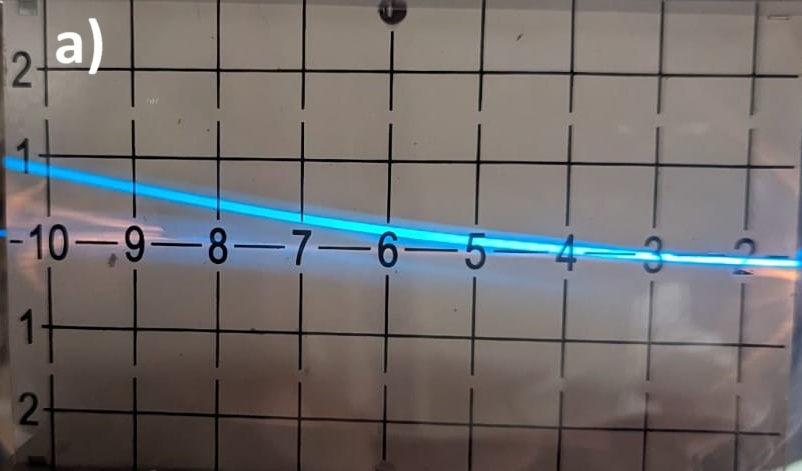
\includegraphics[width=\textwidth]{1kV.jpg}
    \end{minipage}
    \begin{minipage}{0.38\textwidth}
        \centering
        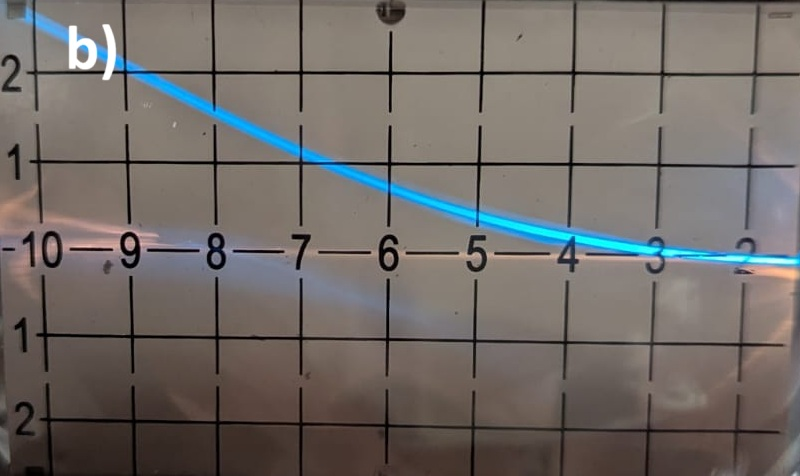
\includegraphics[width=\textwidth]{2kV.jpg}
    \end{minipage}
    \begin{minipage}{0.38\textwidth}
        \centering
        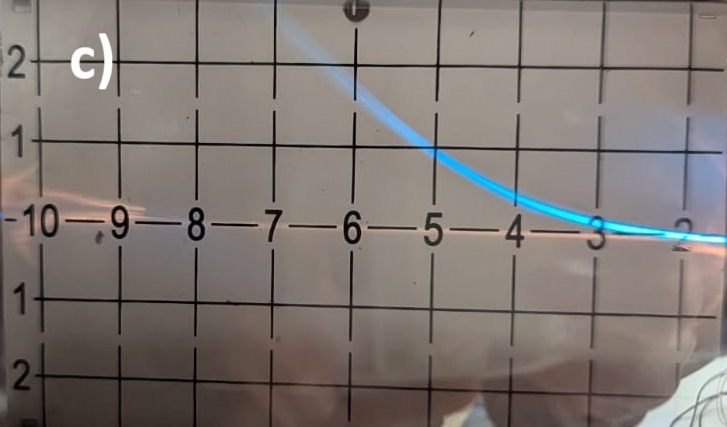
\includegraphics[width=\textwidth]{3kV.jpg}
    \end{minipage}
    \begin{minipage}{0.38\textwidth}
        \centering
        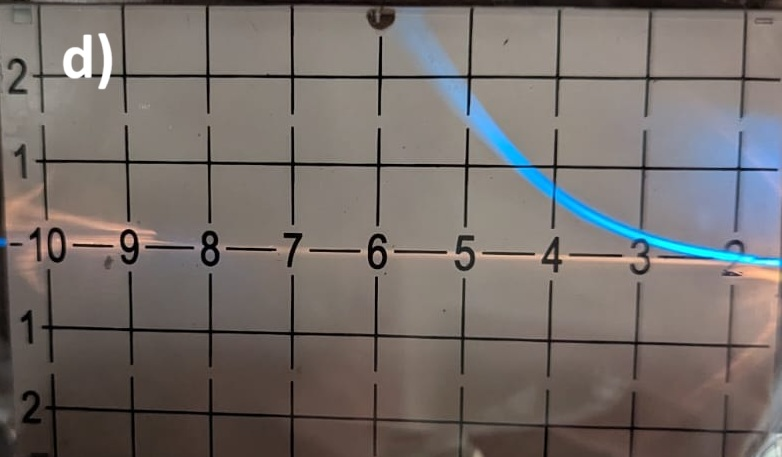
\includegraphics[width=\textwidth]{4kV.jpg}
    \end{minipage}
    \caption{Desviació del raigs en presència del camp elèctric generat per les plàques. (a) 1kV, (b) 2kV, (c) 3kV, (d) 4kV}
    \label{fig: Desv E}
\end{figure}



\section{Càlcul d'incerteses}\label{sec: incerteses}
\underline{Incertesa instrumental:} Hem agafat $\sigma_{c}=\pm0.01A$ i $\sigma_{t}=\pm100V$ com les incerteses de la font de corrent i la font de tensió respectivament. Per altra banda, hem agafat la mitjana del gruix del raig catòdic com  l'incertesa en la mesura dels punts de la trajectòria, ja que per trobar els punts hem usat un mètode de processat d'imatge molt exacte. Això d'ona una incertesa de les mesures de posició: $\sigma_{l}=\pm0.0014m$.

\underline{Propagació d'errors:} Per trobar les incerteses de magnituds dependents d'altres magnituds mesurables hem usat l'equació de propagació d'incerteses
\begin{equation}
    \sigma_{y}^2=\sum_{i=1}^{N}(\frac{\partial y}{\partial x_i})^2\sigma_{x_i}^2
\end{equation}
on y és la manitud dependent i ${x_i}$ les variables mesurables.

Per l'incertesa de la constant k (Equació (\ref{eq: k}))

 \begin{equation}
     \sigma^2_k=\bigg(\frac{4dV_a}{V_p}\bigg)^2\sigma_m^2 + \bigg(\frac{4md}{V_p}\bigg)^2\sigma_{V_a}^2+\bigg(\frac{4mdV_a}{V_p^2}\bigg)^2\sigma_{V_p}^2
 \end{equation}

Per l'incertesa instrumental del radi (Equació (\ref{eq: radi}))
\begin{equation}
    \sigma_{R,ins}^2 = (\frac{\partial R(x,y)}{\partial x})^2+(\frac{\partial R(x,y)}{\partial y})^2= \sigma_{l}^2\bigg[(\frac{x}{y})^2(1-\frac{(x^2+y^2)}{2y^2}^2)\bigg]
    \label{eq: ins_r}
\end{equation}

En el cas del càlcul de l'incertesa dels radis, hem calculat l'incertesa combinada 
\begin{equation}
    \sigma_{R}=\sqrt{\sigma_{R,ins}^2+\sigma_{R,est}^2}
\end{equation}
on $\sigma_{R,ins}$ és l'incertesa instrumental trobada amb l'equació (\ref{eq: ins_r}) evaluada als valors mitjans de $y$ i $x$ de cada corba i $\sigma_{R,est}$ l'incertesa estadística del pendent calculada amb la regressió que hem usat per trobar el radi.

\section{Regressions lineals} \label{sec: Reg}

 Per fer regressions lineals que tenen en compte les incerteces individuals de cadascún dels punt hem utilitzat el mètode de mínims quadrats ponderats (weighted least squares).
 
 Donada una funció $f(x,\vec{\beta})$ a ajustar (en el nostre cas $f(x) = mx+n$):
 \begin{equation}
     f(x,\vec{\beta}) = \sum_{j=1}^m\beta_j\phi_j(x)
 \end{equation}
 
  On ${\beta_j}$ són els paràmetres a ajustar i $\phi_j$ són funcions de x (en el nostre cas $\phi_1 = x$, $\beta_1 = m$ i $\phi_2 = 1$, $\beta_2 = n$)
 
 \begin{equation}
     \hat{\beta} = (X^TWX)^{-1}X^TW\vec{y}
 \end{equation}
 \begin{equation}
     M^\beta = (X^TWX)^{-1}
 \end{equation}
 
 On $\hat{\beta}$ és l'estimador de $\beta$, $M^\beta$ la matriu de variància dels estimadors, d'on els elements de la diagonal són la desviació estàndard al quadrat dels estimadors i, per tant, l'incertesa és l'arrel quadrada dels elements de la diagonal. $W$ és la matriu (diagonal) de ponderació, $X$ és la matriu de les variables independents i $\vec{y}$ el vector de la variable dependent.
 
 \begin{equation}
     W_{ii} = \frac{1}{\sigma_i^2}
 \end{equation}
 \begin{equation}
     X_{ij} = \phi_j(x_i)
 \end{equation}

\section{Trajectòria rectilinia amb camp elèctric i camp magnètic aplicat}\label{sec: traj_no_rect}

Notem que aquesta trajectòria de fet, no és igual de rectílina a la trajectòria que podem observar quan no hi ha aplicat ni camp elèctric ni camp magnètic. Això és degut a la no uniformitat que suposem tant del camp elèctric com del camp magnètic. 

Per una banda el condensador no és ideal, ja que les plaques són petites, lluny de poder-se considerar infinites però és cert que aquests efectes de vorada ja els tenim en compte al calcular la seva $k$ mitjançant la regressió lineal. 

D'altra banda, el solenoide emprat no és ideal tampoc, ja que la seva longitud no és molt més gran que el radi. Això implica que el camp en l'interior sigui de magnitud més gran com més aprop de l'eix central de la bobina ens trobem. Aquest és l'efecte que podem observar en les imatges, podem veure com la trjaectòria dels raigs catòdics presenta més desviació deguda al camp magnètic quan passa pel centre del solenoide.
\end{document}
